\subsection{THE TOPOLOGY OF C}

The mapping \((x, y) \to x + iy\) of the real plane \(R^{2}\) onto C is bijective; by means of this bijection we can transport to C the topology of \(R^{2}\) (cf.~Chapter VI, § 1, no. 5). The topology thus defined on C is compatible with the field structure of C (Chapter III, § 6, no. 7), because it is compatible with the ring structure of C (Chapter VI, § 1, no. 5) and, by (3), 1/z is continuous on the complement \(C^{*}\) of o in C.

If we endow the set C with this topology and with the field structure defined earlier (no. 1, Definition 1), we have defined on C the structure of a topological field (Chapter III, § 6, no. 7); whenever we speak of the topology of C it will always be the above topology that is meant.

In the future we shall generally identify the sets C and \(R^{2}\) considered as topological spaces; the subfield R of C is then identified with the abscissa of \(R^{2}\) , which for this reason is called the real axis; likewise the ordinate is called the imaginary axis (note that this is not a subfield of C). The ray with origin o and direction ratios (1, o) (identified with \(R_{+}\) ) is called the positive real semi-axis; the opposite ray, with the same origin and direction ratios (-1, o), is called the negative real semi-axis.

For the purposes of graphical illustration we use the representation of \(R^{2}\) (well known in elementary analytic geometry) by the points of a plane in which have been drawn two perpendicular coordinate axes, representing respectively the real axis and the imaginary axis of C (Fig. 7).

As in every topological field, every rational function of n complex variables with complex coefficients is continuous at every point of \(C^{n}\) at which the denominator does not vanish.

\pandocbounded{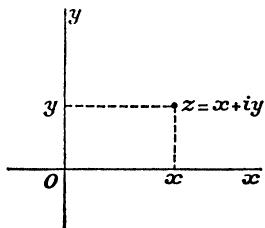
\includegraphics[keepaspectratio]{images/part001_cf49e1ad.jpg}}\\
Figure 7.

The permutation \(z' \to \overline{z}\) of \(\mathbf{C}\) is continuous, and is therefore an automorphism of the topological field \(\mathbf{C}\) .

In fact it is the only automorphism of the topological field C other than the identity automorphism (see Exercise 4).

The functions \(\mathcal{R}(z)\) , \(\mathfrak{J}(z)\) are just the projections of \(\mathbf{R}^2\) onto its factors, and are therefore continuous; the same is true of the absolute value \(|z|\) , since it is the Euclidean norm (Chapter VI, § 2, no. 1) of the point \((x,y)\) in \(\mathbf{R}^2\) .

The properties of the absolute value lead to another proof of the fact that the topology of \(\mathbf{C}\) is compatible with its field structure (cf.~Chapter IX, § 3, no. 2); the continuity of \(z + z'\) follows from the triangle inequality \(|z + z'| \leqslant |z| + |z'|\) ; that of \(zz'\) follows from the relation

\[
\begin{array}{r l} | z z ^ {\prime} - z _ {0} z _ {0} ^ {\prime} | & = | z _ {0} (z ^ {\prime} - z _ {0} ^ {\prime}) + (z - z _ {0}) z _ {0} ^ {\prime} + (z - z _ {0}) (z ^ {\prime} - z _ {0} ^ {\prime}) | \\ & \leqslant | z _ {0} | \cdot | z ^ {\prime} - z _ {0} ^ {\prime} | + | z _ {0} ^ {\prime} | \cdot | z - z _ {0} | + | z - z _ {0} | \cdot | z ^ {\prime} - z _ {0} ^ {\prime} |; \end{array}
\]

lastly, the continuity of \(z^{-1}\) follows from the relation

\[
\left| z _ {0} ^ {- 1} - z ^ {- 1} \right| = | z | ^ {- 1}. \left| z - z _ {0} \right|. \left| z _ {0} \right| ^ {- 1}.
\]

